\documentclass[conference]{IEEEtran}
\IEEEoverridecommandlockouts
\usepackage{cite}
\usepackage{amsmath,amssymb}
\usepackage{graphicx}
\graphicspath{{figures/}}
\usepackage{booktabs}
\usepackage{threeparttable}
\usepackage{multirow}

% ---------------------------------------------------------------
% EDIT BEFORE SUBMISSION: technology node used for the simulations
\newcommand{\TECH}{10-nm}
% ---------------------------------------------------------------

\begin{document}

\title{Stability and Power Analysis of a Read-Decoupled 8T SRAM Cell in 10-nm Technology and Power Optimization Using a Diode-Clamped Gated-Ground Footer}

\author{\IEEEauthorblockN{S Prajwal}
\IEEEauthorblockA{\textit{School of Electronics Engineering} \\
\textit{Vellore Institute of Technology}\\
Vellore, Tamil Nadu, India \\
prajwal.s2026@vitstudent.ac.in}
}

\maketitle

\begin{abstract}
Static random-access memory (SRAM) dominates the area and standby power of modern systems-on-chip, and the stability of the conventional six-transistor (6T) cell degrades sharply as the supply voltage is reduced. This paper presents the design and characterization of a read-decoupled eight-transistor (8T) SRAM cell at a supply of 0.75\,V, simulated with Cadence Virtuoso and Spectre using 10-nm FinFET predictive models. Butterfly-curve analysis gives a hold static noise margin (HSNM) of 274.5\,mV, a read static noise margin (RSNM) of 274.5\,mV and a write static noise margin (WSNM) of 301.1\,mV, corresponding to 36.6\%, 36.6\% and 40.1\% of $V_{DD}$. Because the read path is isolated from the storage nodes, the read margin equals the hold margin, whereas conventional 6T cells reported in the literature retain only about half of their hold margin during a read. A gated-ground footer with a diode-connected clamp transistor is then added to the cross-coupled core, which lowers the average power from 468.10\,nW to 441.85\,nW (5.6\%) while preserving correct write and read operation. The cell is compared with 6T, 7T and 8T designs from the literature using supply-normalized margins.
\end{abstract}

\begin{IEEEkeywords}
8T SRAM, static noise margin, read stability, write margin, leakage power, gated ground, low-voltage memory
\end{IEEEkeywords}

\section{Introduction}
On-chip SRAM occupies a large and growing share of die area in processors and edge devices, so its leakage and access energy strongly influence total system power. Supply-voltage scaling is the most effective lever for reducing power, because dynamic energy scales with $V_{DD}^2$ and leakage also falls with $V_{DD}$. The conventional 6T cell, however, limits how far $V_{DD}$ can be reduced. During a read, the bitline is connected directly to a storage node through the access transistor, raising the voltage of the node storing `0'. The read static noise margin (RSNM) is therefore considerably smaller than the hold margin, and the transistor sizing that improves read stability degrades writability~\cite{seevinck1987snm}.

Several cell topologies address this conflict. Seven-transistor (7T) cells weaken or remove the read disturb by modifying the feedback loop or the access path, and have been studied down to the 10-nm and 7-nm FinFET nodes~\cite{ansari2015near7t,yang2016single7t}. The 8T cell adds a dedicated two-transistor read port, decoupling read stability from write ability~\cite{chang2005stable}.

This paper makes three contributions. First, it characterizes the hold, read and write stability of a read-decoupled 8T cell at 0.75\,V using butterfly-curve analysis. Second, it compares these margins with 6T, 7T and 8T results from the literature using supply-normalized figures, since the published cells were simulated at different voltages and nodes. Third, it applies a diode-clamped gated-ground footer to the 8T core and quantifies the resulting power reduction.

\section{Device Technology and Simulation Setup}
All circuits use the 10-nm high-performance (HP) multi-gate Predictive Technology Model (PTM-MG)~\cite{sinha2012ptm}, a BSIM-CMG (level~72) FinFET model, simulated with Cadence Virtuoso and Spectre at 27\,$^{\circ}$C. Every transistor uses a single fin. Table~\ref{tab:device} lists the device parameters taken from the NFET and PFET model cards. The threshold voltages are estimated from the gate work function $\phi_G$ relative to the silicon midgap (4.61\,eV), since BSIM-CMG has no explicit $V_{th0}$ parameter.

\begin{table}[t]
\caption{10-nm FinFET Device Parameters (PTM-MG HP)}
\label{tab:device}
\centering
\setlength{\tabcolsep}{3pt}\footnotesize
\begin{tabular}{lcc}
\toprule
\textbf{Parameter} & \textbf{NFET} & \textbf{PFET} \\
\midrule
Gate length, $L$ & 14 nm & 14 nm \\
Fin thickness, $T_{fin}$ & 8 nm & 8 nm \\
Fin height, $H_{fin}$ & 21 nm & 21 nm \\
Fin width, $2H_{fin}+T_{fin}$ & 50 nm & 50 nm \\
No. of fins / fin pitch & 1 / 28 nm & 1 / 28 nm \\
Oxide thickness, $T_{ox}$ (EOT) & 0.68 nm & 0.68 nm \\
Channel doping, $N_{body}$ & $2.5\times10^{16}$ cm$^{-3}$ & $2.5\times10^{16}$ cm$^{-3}$ \\
S/D doping, $N_{SD}$ & $3\times10^{20}$ cm$^{-3}$ & $3\times10^{20}$ cm$^{-3}$ \\
S/D ext. doping, $N_{SDE}$ & $6\times10^{19}$ cm$^{-3}$ & $6\times10^{19}$ cm$^{-3}$ \\
Gate work function, $\phi_G$ & 4.42 eV & 4.75 eV \\
Threshold, $V_{th}$ (est.) & $\approx$ 0.30 V & $\approx -$0.35 V \\
Supply, $V_{DD}$ & 0.75 V & 0.75 V \\
\bottomrule
\end{tabular}
\end{table}

\section{8T SRAM Cell Architecture}

\subsection{Cell Structure}
Fig.~\ref{fig:cell} shows the schematic of the 8T cell. Two cross-coupled inverters store the complementary data $Q$ and $Q_B$. Two NMOS write-access transistors, gated by the write wordline (WWL), connect $Q$ and $Q_B$ to the differential write bitlines WBL and WBLB. The read port consists of two series NMOS transistors: a read-driver transistor whose gate is driven by $Q_B$, and a read-access transistor gated by the read wordline (RWL) that connects the stack to the single-ended read bitline (RBL).

\begin{figure}[t]
\centering
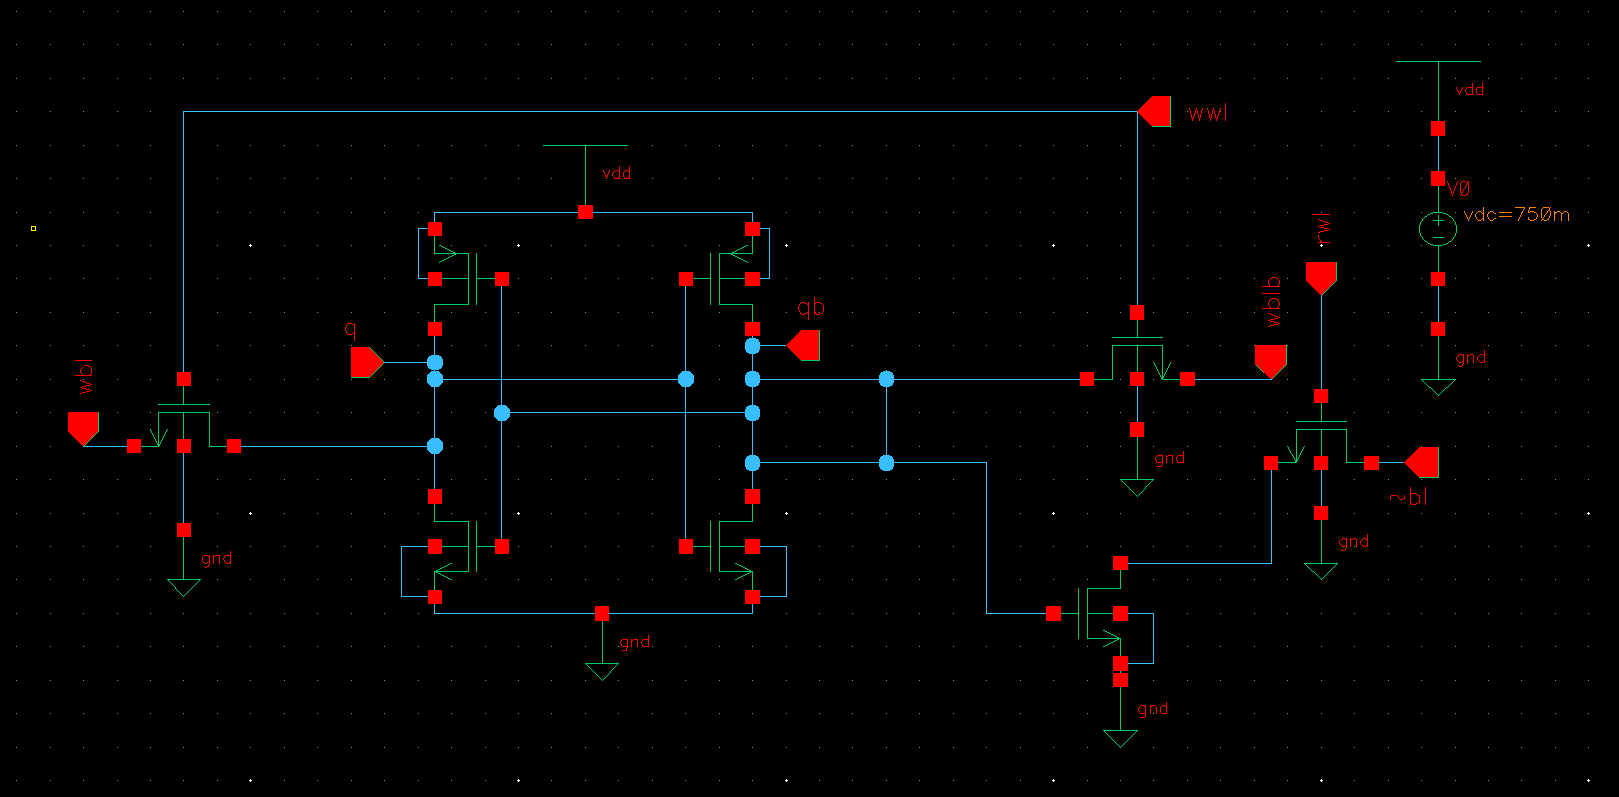
\includegraphics[width=\columnwidth]{8tsramckt.png}
\caption{Schematic of the read-decoupled 8T SRAM cell: 6T storage core with differential write port (WWL, WBL, WBLB) and two-transistor single-ended read port (RWL, RBL).}
\label{fig:cell}
\end{figure}

\subsection{Operation}
\textit{Write:} WBL and WBLB are driven to complementary values and WWL is raised. The write-access transistors overpower the cross-coupled inverters and flip the cell. Because the cell is never read through these transistors, they can be sized for strong writability without degrading read stability.

\textit{Read:} RBL is precharged to $V_{DD}$ by a PMOS precharge transistor, PRE is released, and RWL is raised. If $Q_B$ is high (i.e., $Q=0$), the read stack conducts and discharges RBL. If $Q_B$ is low, RBL remains at $V_{DD}$. The storage nodes drive only the gate of the read-driver transistor, so no current is injected into them during a read. The cell therefore has no read-disturb mechanism, and its read margin approaches its hold margin~\cite{chang2005stable}.

\textit{Hold:} WWL and RWL are held low, and the cross-coupled inverters retain the data.

\section{Stability Analysis}

\subsection{Methodology}
The static noise margins were extracted using the butterfly-curve method~\cite{seevinck1987snm}. Fig.~\ref{fig:snm}(a)--(c) shows the three test benches. In each, the feedback loop of the cross-coupled pair is broken, and a DC source sweeps the input of one inverter from 0 to 0.75\,V while the output of the other inverter is recorded. The two voltage-transfer characteristics are superimposed, and the SNM is taken as the side of the largest square that fits inside the smaller lobe. For HSNM, all wordlines are low. For RSNM, the read port is biased in its read condition with the read bitline held at $V_{DD}$. For WSNM, the cell is biased in the write condition. All sweeps use $V_{DD}=0.75$\,V.

\begin{figure*}[t]
\centering
\begin{minipage}{0.325\textwidth}\centering
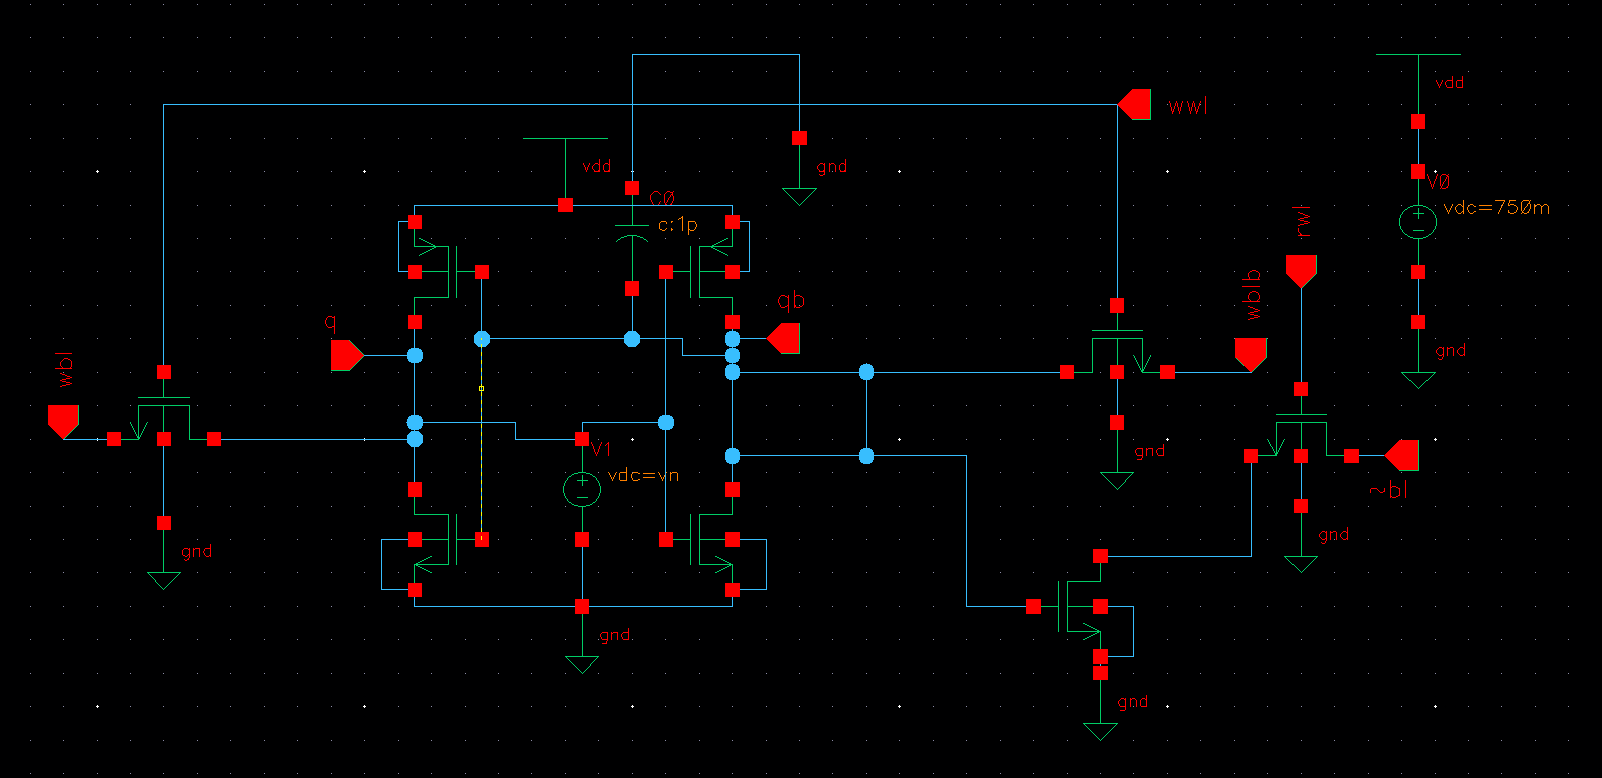
\includegraphics[width=\linewidth]{holdsramckt.png}\\[-1pt]
\footnotesize (a) Hold test bench
\end{minipage}\hfill
\begin{minipage}{0.325\textwidth}\centering
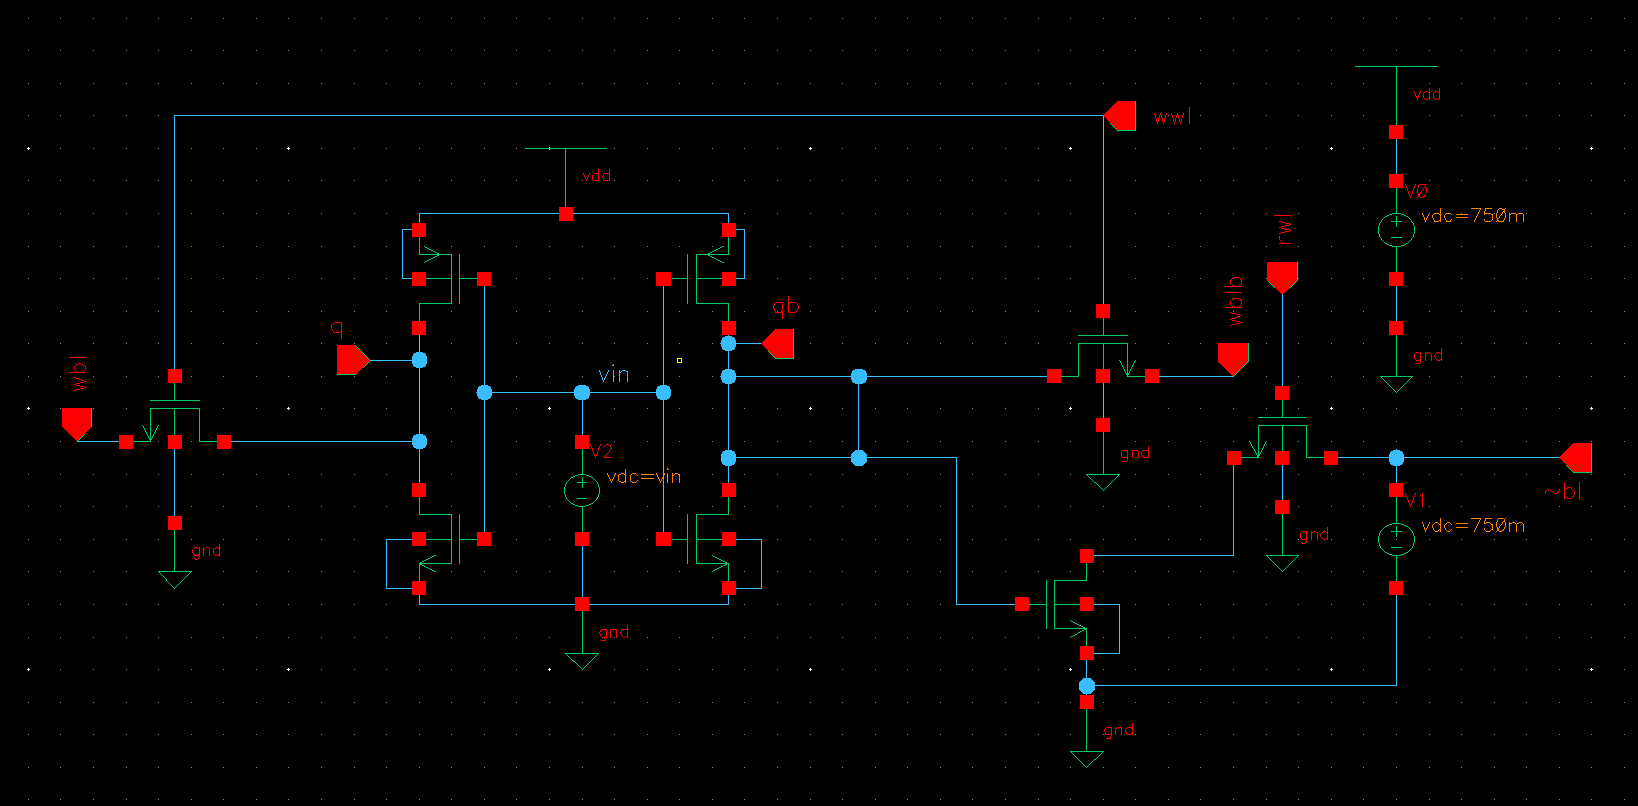
\includegraphics[width=\linewidth]{readsramckt.png}\\[-1pt]
\footnotesize (b) Read test bench
\end{minipage}\hfill
\begin{minipage}{0.325\textwidth}\centering
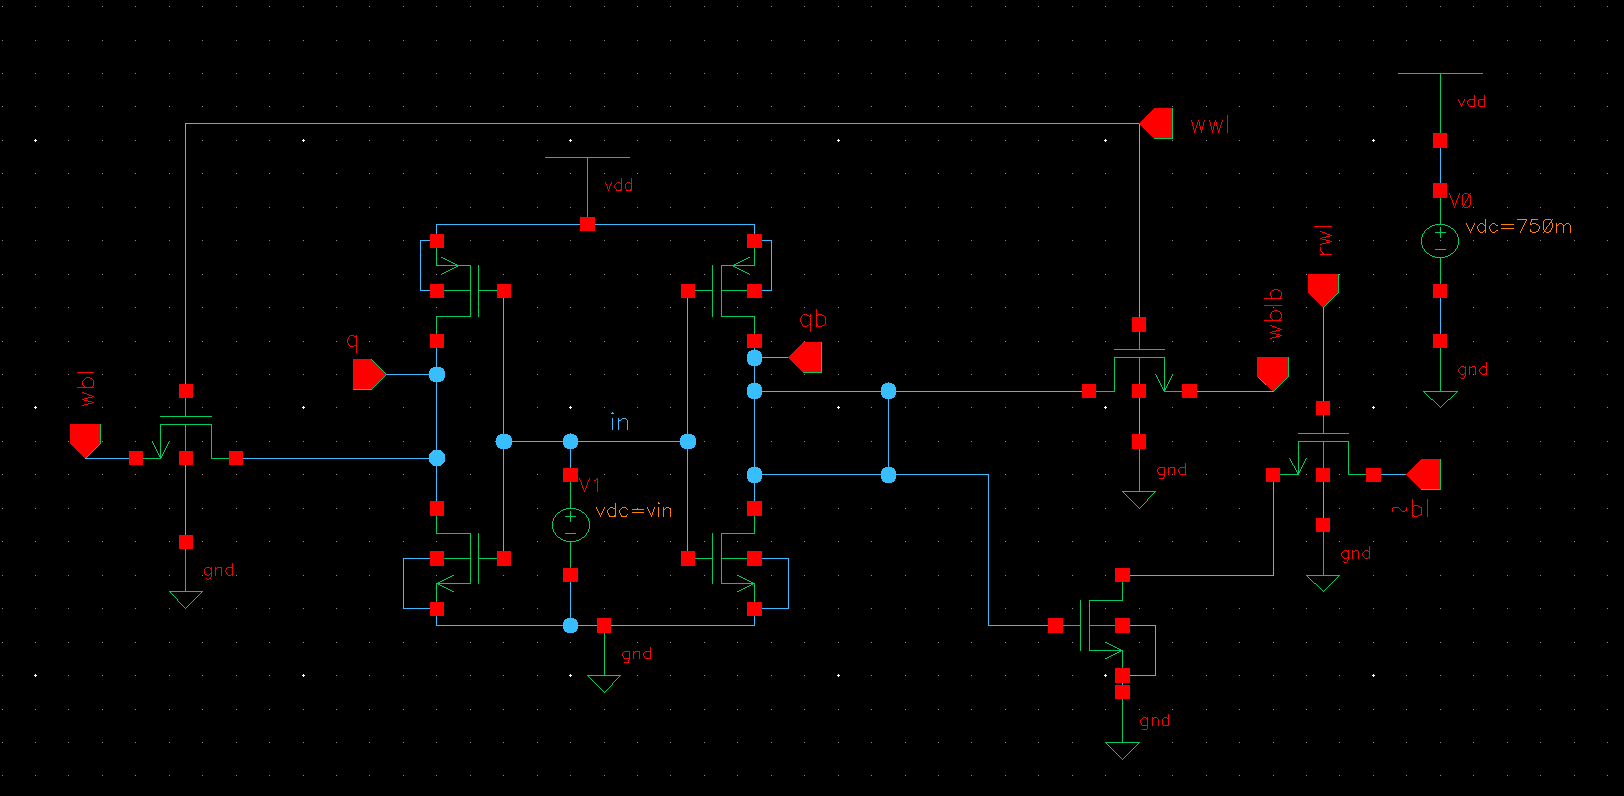
\includegraphics[width=\linewidth]{writesramckt.png}\\[-1pt]
\footnotesize (c) Write test bench
\end{minipage}\\[4pt]
\begin{minipage}{0.325\textwidth}\centering
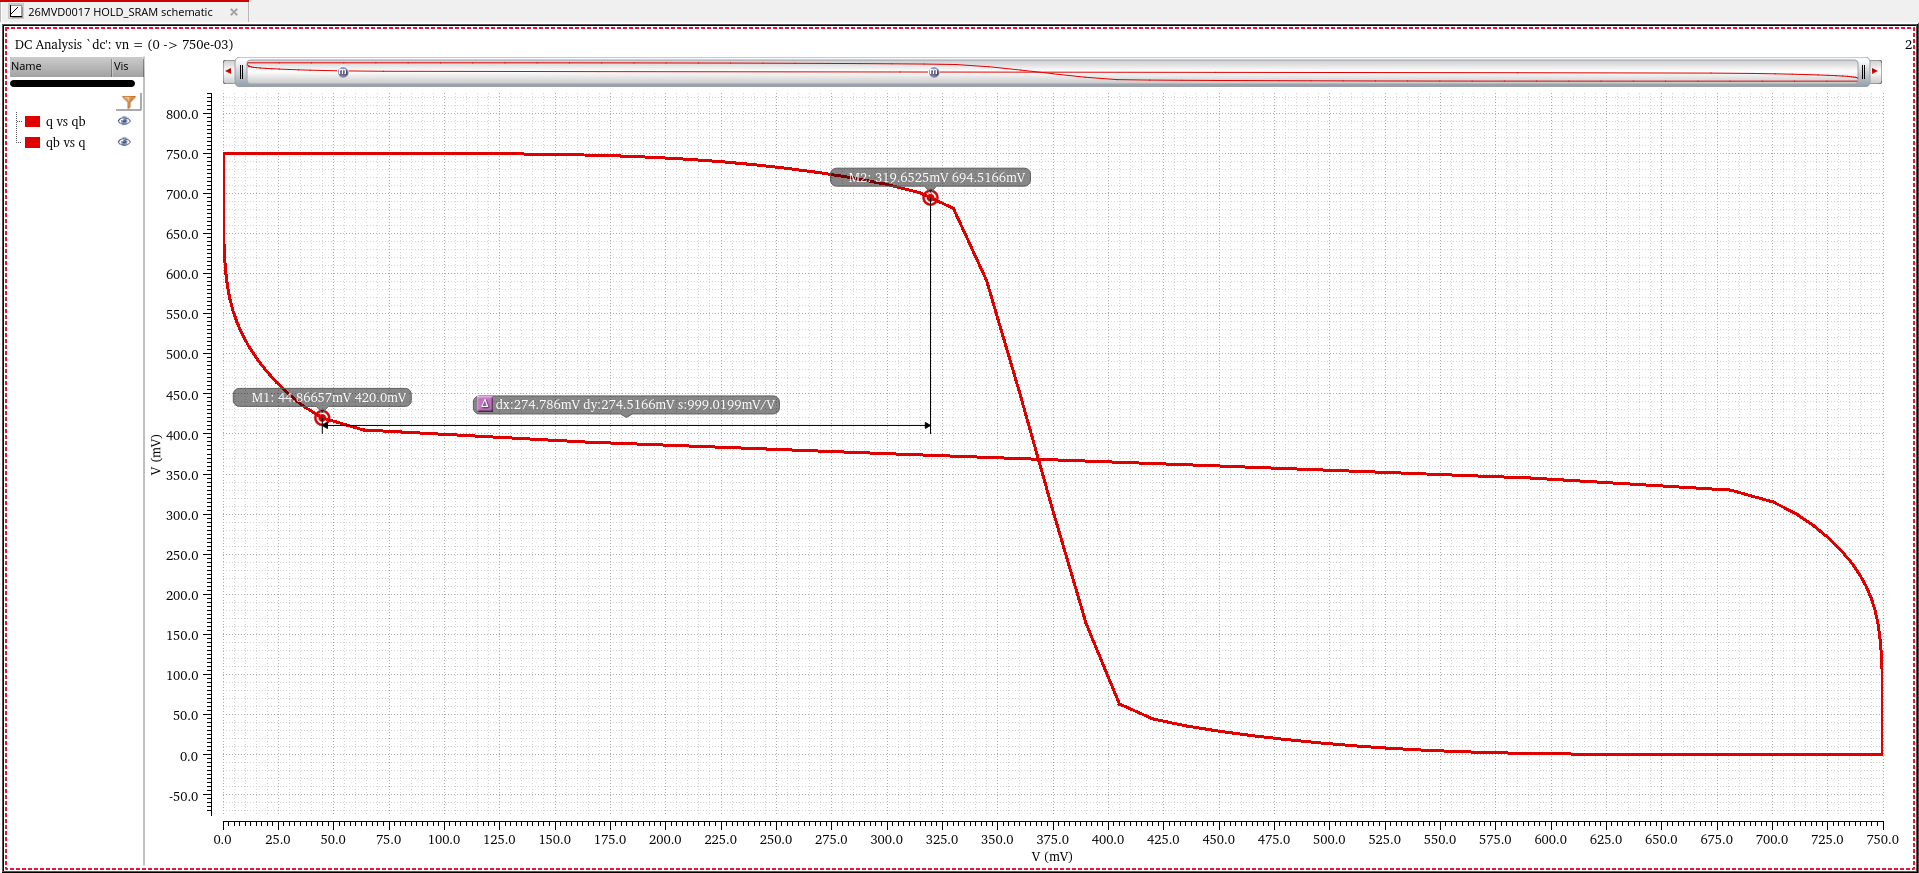
\includegraphics[width=\linewidth]{hold_margin.png}\\[-1pt]
\footnotesize (d) Hold butterfly curve
\end{minipage}\hfill
\begin{minipage}{0.325\textwidth}\centering
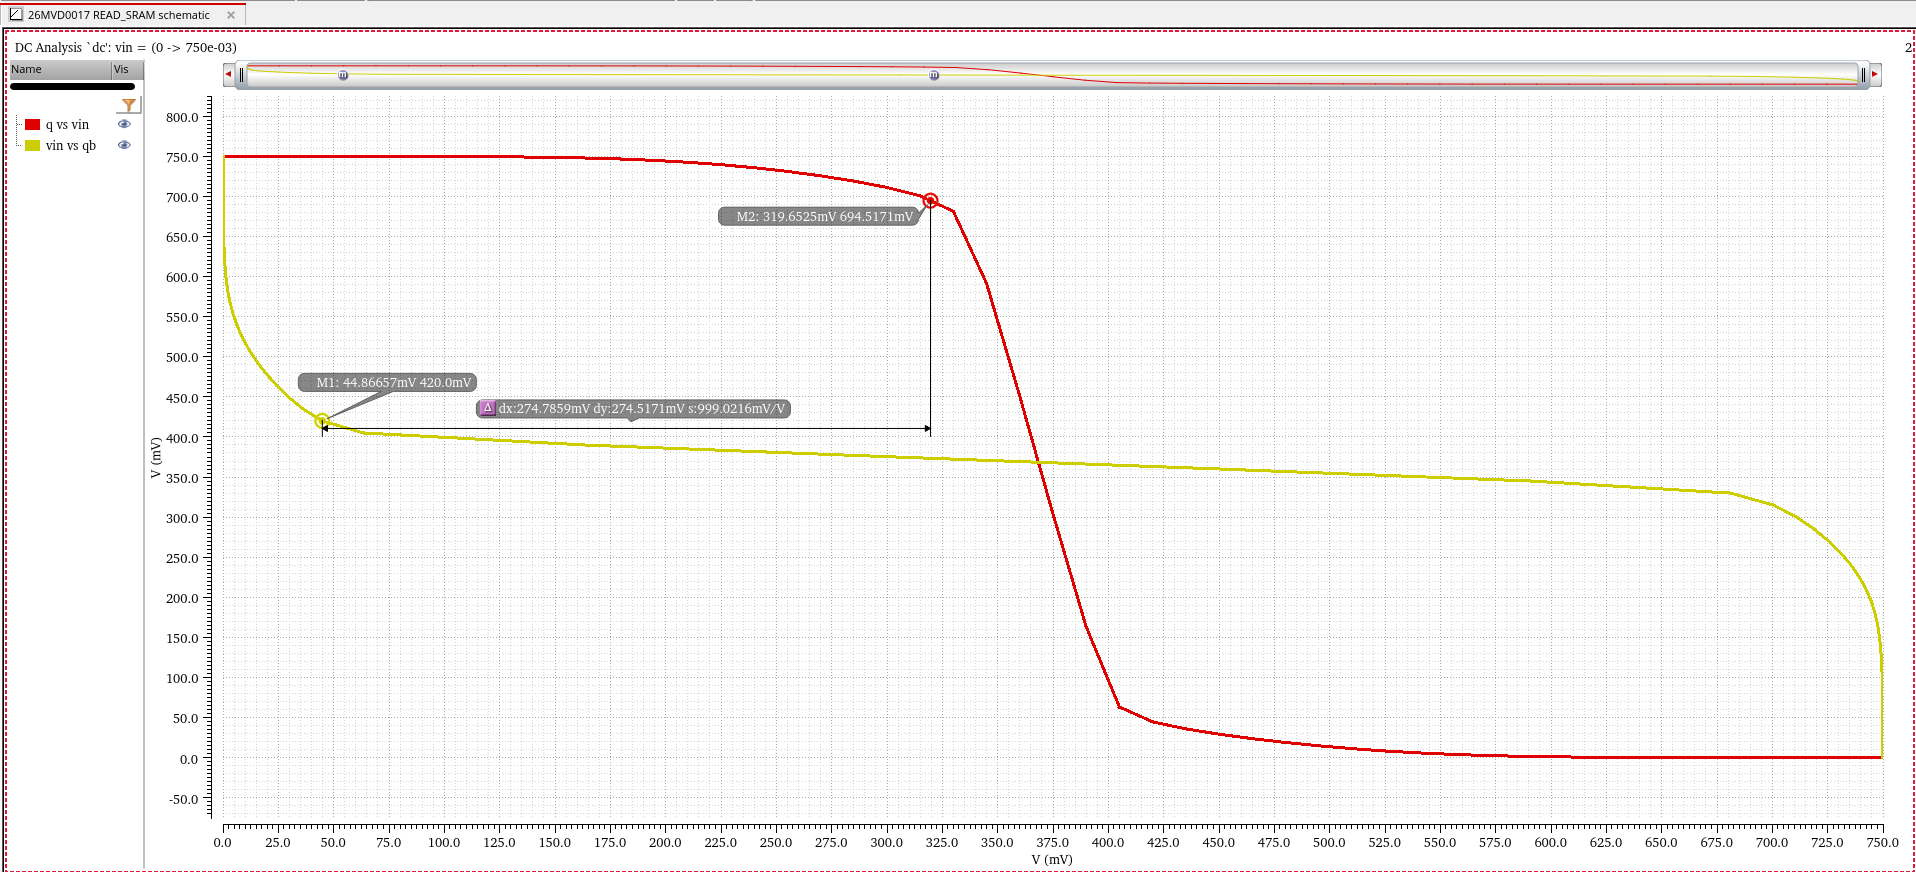
\includegraphics[width=\linewidth]{read_margin.png}\\[-1pt]
\footnotesize (e) Read butterfly curve
\end{minipage}\hfill
\begin{minipage}{0.325\textwidth}\centering
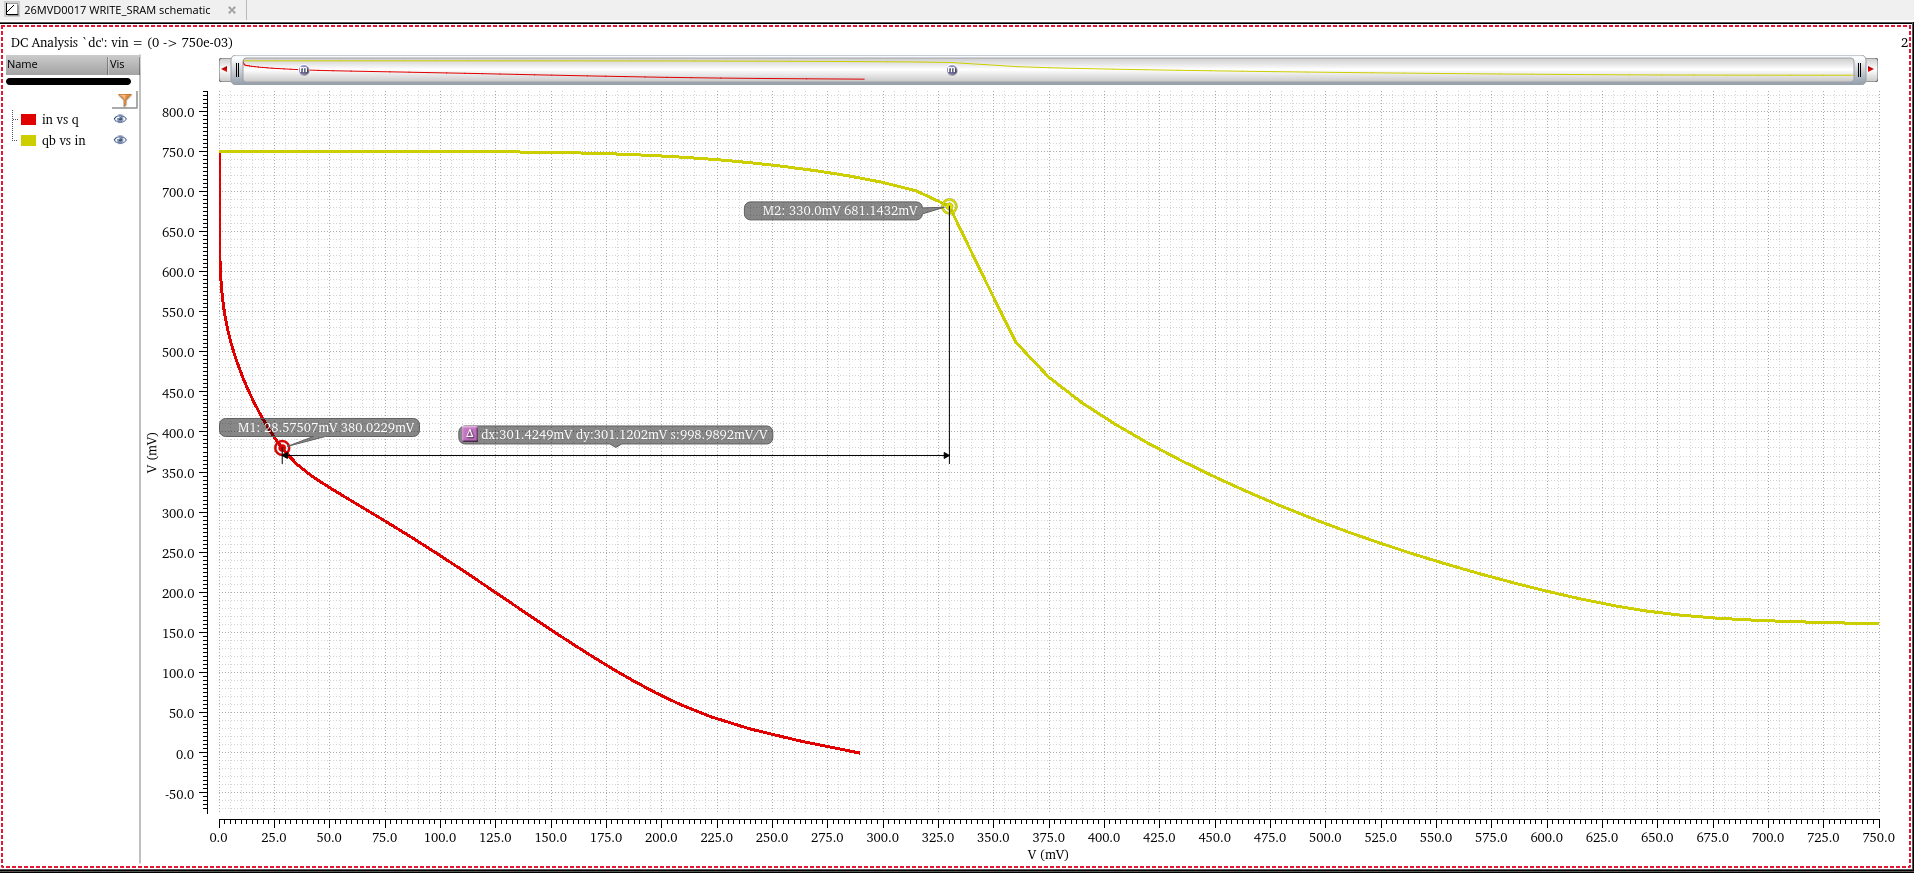
\includegraphics[width=\linewidth]{write_margin.png}\\[-1pt]
\footnotesize (f) Write butterfly curve
\end{minipage}
\caption{Static noise margin test benches (a)--(c) and the corresponding butterfly curves (d)--(f) at $V_{DD}=0.75$\,V: HSNM $=274.5$\,mV, RSNM $=274.5$\,mV, WSNM $=301.1$\,mV.}
\label{fig:snm}
\end{figure*}

\subsection{Hold and Read Margins}
Fig.~\ref{fig:snm}(d) shows the hold butterfly curve. The largest inscribed square, bounded by markers at (44.9\,mV, 420.0\,mV) and (319.7\,mV, 694.5\,mV), has sides of $\Delta x = 274.8$\,mV and $\Delta y = 274.5$\,mV, giving HSNM $=274.5$\,mV, or 36.6\% of $V_{DD}$.

Fig.~\ref{fig:snm}(e) shows the read butterfly curve. Its inscribed square is identical to within 0.1\,mV ($\Delta x = 274.8$\,mV, $\Delta y = 274.5$\,mV), giving RSNM $=274.5$\,mV. The ratio RSNM/HSNM is therefore 1.00, which confirms that activating the read port does not disturb the storage nodes. In a 6T cell, by contrast, the access transistor and pull-down transistor form a voltage divider during a read, which raises the `0' node and shrinks one lobe of the butterfly.

\subsection{Write Margin}
Fig.~\ref{fig:snm}(f) shows the write-mode curves. In the write condition, the transfer characteristic of the inverter whose node is being pulled low collapses, leaving a single large lobe. The inscribed square, bounded by markers at (28.6\,mV, 380.0\,mV) and (330.0\,mV, 681.1\,mV), has sides of $\Delta x = 301.4$\,mV and $\Delta y = 301.1$\,mV, giving WSNM $=301.1$\,mV, or 40.1\% of $V_{DD}$. A larger WSNM indicates that the write drivers can flip the cell with more tolerance to variation. Because the read port is separate, the write-access transistors could be strengthened further to raise WSNM without any penalty on RSNM.

\section{Transient Verification}
The functionality of the cell was verified with a 2-ns transient simulation that included the precharge transistor and a 1-fF RBL load capacitance (Fig.~\ref{fig:tran}). The sequence is as follows:
\begin{itemize}
\item \textbf{Write `1' (0.2--0.3\,ns):} WBL is high and WWL is pulsed. $Q$ rises to $V_{DD}$ and $Q_B$ falls to 0.
\item \textbf{Read `1' (0.6--0.7\,ns):} PRE is released and RWL is pulsed. Because $Q_B=0$, the read driver is off and RBL stays at $V_{DD}$.
\item \textbf{Write `0' (1.2--1.3\,ns):} WBL is low and WWL is pulsed. $Q$ falls to 0 and $Q_B$ rises to $V_{DD}$.
\item \textbf{Read `0' (1.6--1.7\,ns):} With $Q_B$ high, the read stack conducts and RBL discharges to nearly 0\,V within about 30\,ps. RBL is restored to $V_{DD}$ when PRE returns low.
\end{itemize}
Throughout both read operations, $Q$ and $Q_B$ show no visible disturbance, consistent with the equal hold and read margins.

\begin{figure}[t]
\centering
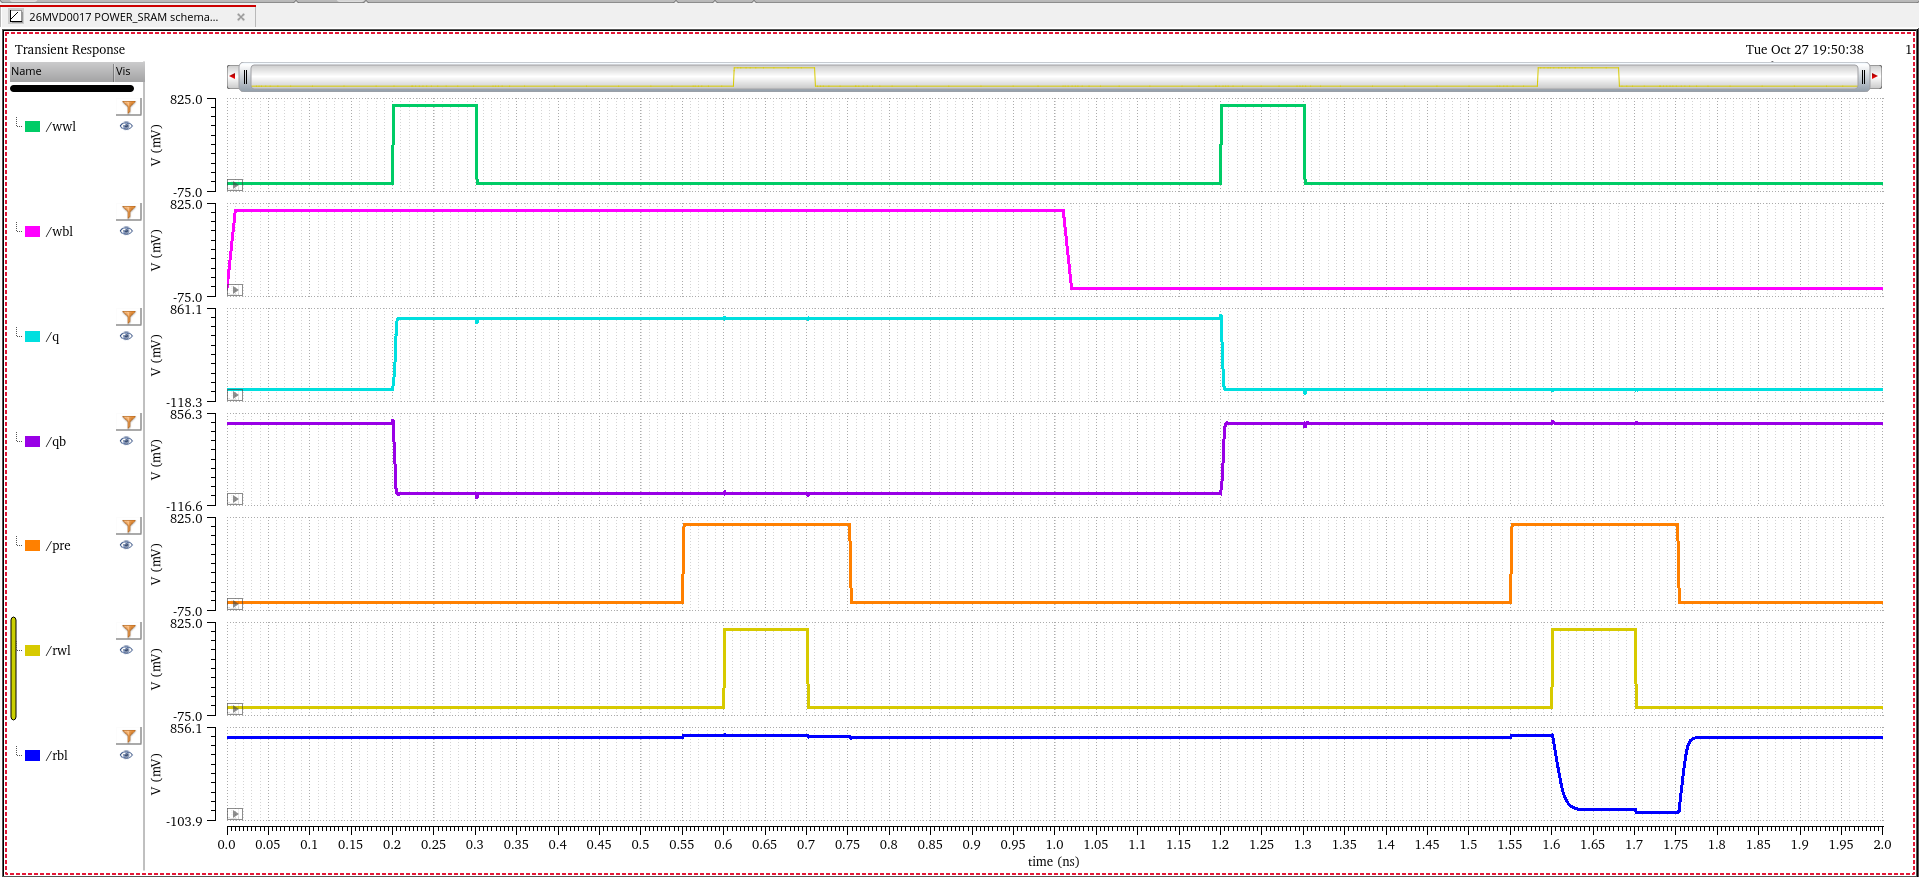
\includegraphics[width=\columnwidth]{TransientAnalysis.png}
\caption{Transient response over 2\,ns (top to bottom: WWL, WBL, $Q$, $Q_B$, PRE, RWL, RBL), showing write `1', read `1', write `0' and read `0'.}
\label{fig:tran}
\end{figure}

\section{Power Optimization Using a Diode-Clamped Gated-Ground Footer}

\subsection{Technique}
Subthreshold leakage through the cross-coupled inverters is a major component of SRAM power, particularly when most cells in an array are idle. Gated-ground techniques insert a high-resistance device in the ground path of idle cells to suppress this leakage~\cite{agarwal2003gatedground}. A plain footer, however, lets the virtual ground float toward $V_{DD}$ in sleep mode, which destroys the stored data.

Fig.~\ref{fig:pwrckt}(a) shows the power test bench of the conventional 8T cell, with the PMOS precharge transistor and a 1-fF RBL load. Fig.~\ref{fig:pwrckt}(b) shows the modified cell. The sources of the two pull-down transistors are tied to a virtual ground node, VGND, which connects to ground through two parallel NMOS devices. The first is a sleep transistor gated by SLEEPB. It is on in active mode, giving a low-resistance path, and off in sleep mode. The second is a diode-connected NMOS whose gate and drain are both tied to VGND. In sleep mode it clamps VGND to approximately one threshold voltage above ground. The cell then retains its data with a reduced effective supply of about $V_{DD}-V_{th}$, while the stacking effect and the negative gate-source voltage seen by the off pull-down transistors reduce leakage through the core~\cite{agarwal2003gatedground}. The read port remains referenced to the true ground, so read current and RBL discharge speed are not degraded by the footer.

\begin{figure*}[t]
\centering
\begin{minipage}{0.49\textwidth}\centering
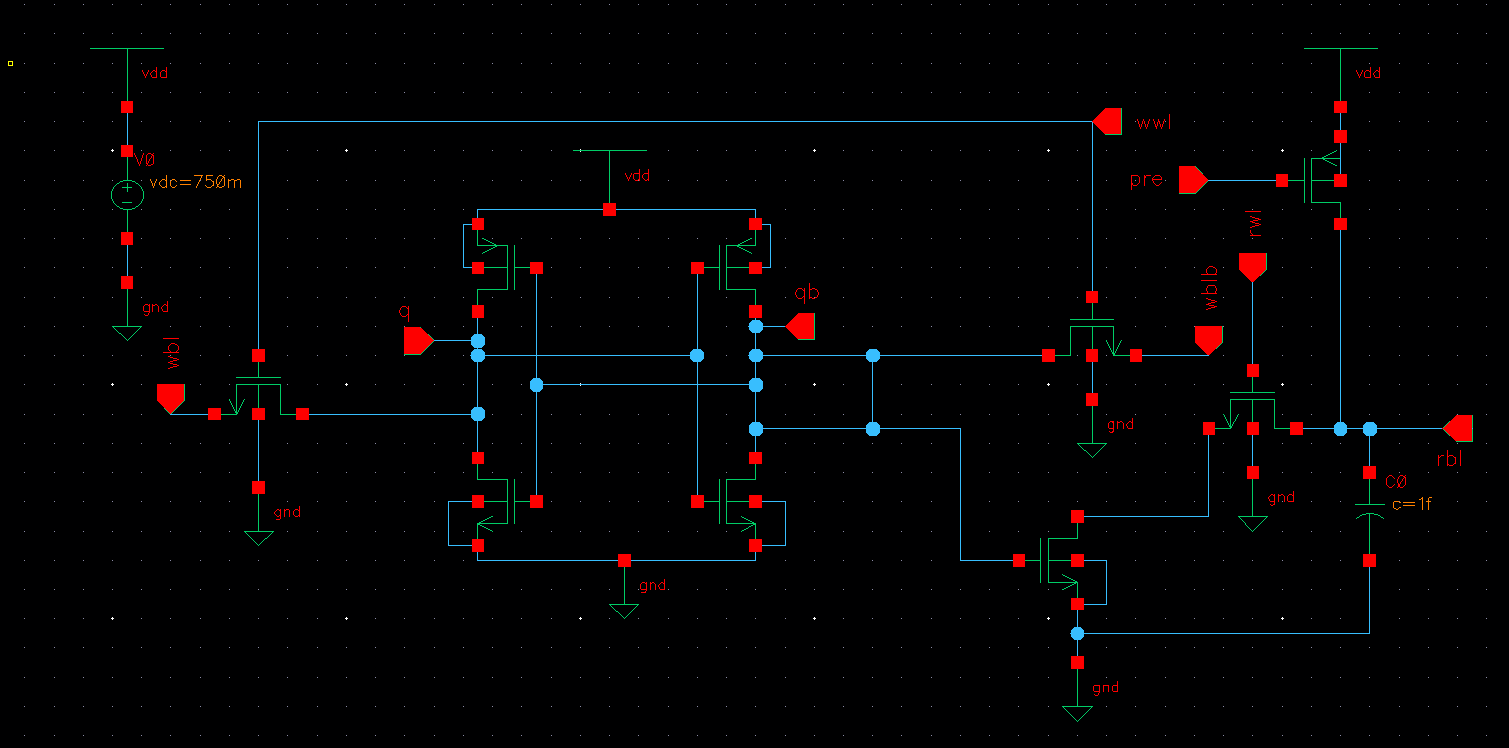
\includegraphics[width=\linewidth]{poweranalysis.png}\\[-1pt]
\footnotesize (a) Conventional 8T cell
\end{minipage}\hfill
\begin{minipage}{0.49\textwidth}\centering
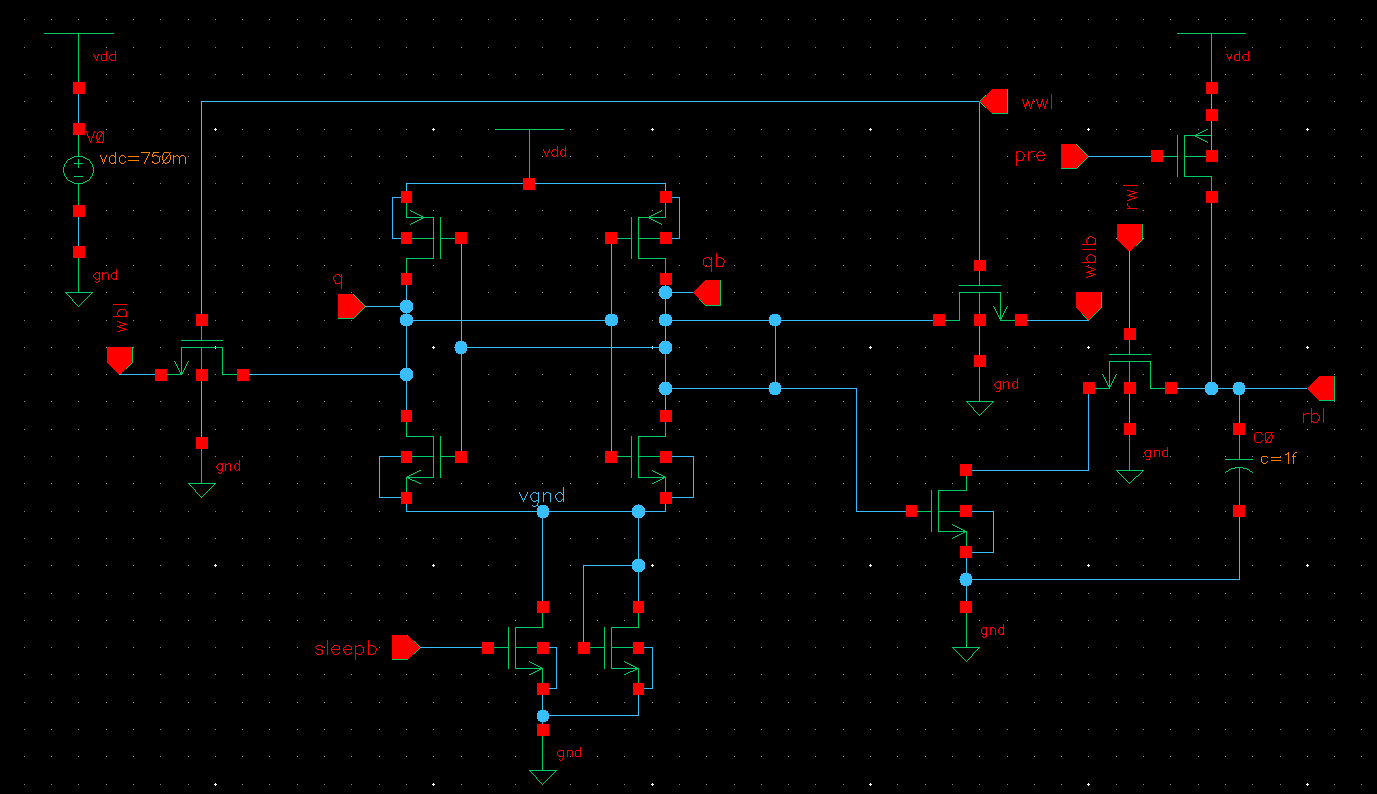
\includegraphics[width=\linewidth]{poweranalysisoptimised.png}\\[-1pt]
\footnotesize (b) 8T cell with diode-clamped gated-ground footer
\end{minipage}
\caption{Power-analysis test benches. In (b) the pull-down network returns through VGND, which connects to ground through a sleep transistor (SLEEPB) in parallel with a diode-connected clamp transistor.}
\label{fig:pwrckt}
\end{figure*}

\subsection{Results}
The average power drawn from the 0.75-V supply was measured in Cadence ADE over the same 2-ns write/read sequence for both versions of the cell (Fig.~\ref{fig:pwr}). The footer lowers the average power from 468.10\,nW to 441.85\,nW, a reduction of 26.26\,nW or 5.6\%. The functional waveforms remain correct. The saving in this measurement comes from the leakage reduction during the idle portions of the sequence. Larger savings are expected in standby-dominated operation, where the cell spends most of its time in sleep mode.

\begin{figure}[t]
\centering
\begin{minipage}{0.49\columnwidth}\centering
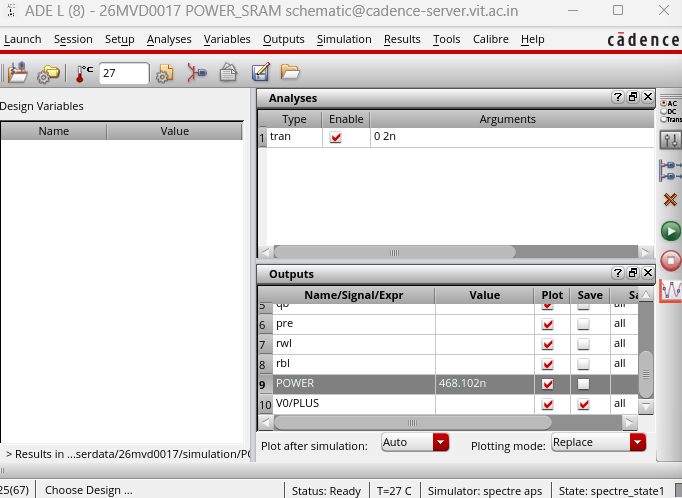
\includegraphics[width=\linewidth]{power.png}\\[-1pt]
\footnotesize (a) Conventional: 468.102\,nW
\end{minipage}\hfill
\begin{minipage}{0.49\columnwidth}\centering
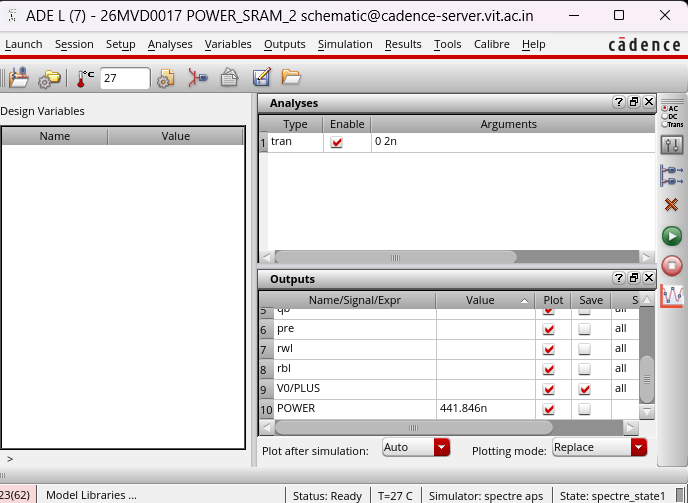
\includegraphics[width=\linewidth]{power_optimised.png}\\[-1pt]
\footnotesize (b) With footer: 441.846\,nW
\end{minipage}
\caption{Average power reported by Cadence ADE over the 2-ns transient.}
\label{fig:pwr}
\end{figure}



\section{Comparison with 6T and 7T Cells}
Table~\ref{tab:compare} compares this work with FinFET SRAM cells simulated at nearby nodes using the same PTM-MG model family. Part~A lists the noise margins reported for 6T and 8T cells at 7~nm~\cite{abbasian2022comp}. Part~B lists the minimum operating voltage ($V_{min}$) of 6T, 7T and 8T cells at 10~nm~\cite{ansari2015near7t}, together with the margin that limits it. Because the supplies differ, two supply-independent figures are used: RSNM normalized to $V_{DD}$, and the RSNM/HSNM ratio.

\begin{table*}[t]
\centering
\begin{threeparttable}
\caption{Comparison with Reported FinFET 6T, 7T and 8T SRAM Cells (PTM-MG Models)}
\label{tab:compare}
\begin{tabular}{llccccccc}
\toprule
\textbf{Ref.} & \textbf{Cell} & \textbf{Node} & \textbf{$V_{DD}$ (V)} & \textbf{HSNM (mV)} & \textbf{RSNM (mV)} & \textbf{WSNM (mV)} & \textbf{RSNM/$V_{DD}$} & \textbf{RSNM/HSNM} \\
\midrule
\multicolumn{9}{l}{\textit{A. Noise margins}} \\
\cite{abbasian2022comp} & 6T & 7 nm & 0.20 & 67.1 & 32.8 & 73.4 & 16.4\% & 0.49 \\
\cite{abbasian2022comp} & 8T & 7 nm & 0.20 & 67.1 & 67.1 & 46.9 & 33.6\% & 1.00 \\
\midrule
\multicolumn{9}{l}{\textit{B. Minimum operating voltage at 10 nm (limiting margin)}} \\
\cite{ansari2015near7t} & 6T-HP & 10 nm & $V_{min}=0.50$ & \multicolumn{5}{l}{limited by RSNM (read disturb)} \\
\cite{ansari2015near7t} & 7T & 10 nm & $V_{min}=0.40$ & \multicolumn{5}{l}{limited by HSNM} \\
\cite{ansari2015near7t} & 8T-HP & 10 nm & $V_{min}=0.32$ & \multicolumn{5}{l}{limited by write margin} \\
\midrule
\textbf{This work} & \textbf{8T} & \textbf{10 nm} & \textbf{0.75} & \textbf{274.5} & \textbf{274.5} & \textbf{301.1} & \textbf{36.6\%} & \textbf{1.00} \\
\bottomrule
\end{tabular}
\begin{tablenotes}\footnotesize
\item HP: high-performance variant. Ref.~\cite{ansari2015near7t} reports margins only graphically; $V_{min}$ values are from its tabulated results.
\end{tablenotes}
\end{threeparttable}
\end{table*}

Three observations follow from the comparison.

\textit{Read stability.} At 7~nm, the 6T cell retains only 49\% of its hold margin during a read, while the 8T cell retains 100\%~\cite{abbasian2022comp}. This work confirms the same behaviour at 10~nm, with RSNM/HSNM $=1.00$. At 10~nm, the 6T-HP cell is the only cell whose $V_{min}$ is set by the read margin~\cite{ansari2015near7t}, which is exactly the limitation the decoupled read port removes. The normalized RSNM of this work, 36.6\% of $V_{DD}$, is about 2.2 times that of the 7-nm 6T cell.

\textit{Comparison with 7T.} The 10-nm 7T cell removes the read disturb, so its $V_{min}$ of 0.40\,V is limited by hold stability rather than by the read margin~\cite{ansari2015near7t}. It improves on the 6T-HP cell (0.50\,V), but the 8T-HP cell reaches a lower $V_{min}$ of 0.32\,V. 7T designs also rely on extra control, such as a transmission gate that isolates the bitline or a two-phase write for a `1'~\cite{yang2016single7t}, whereas the 8T cell keeps the standard differential write path.

\textit{Write ability.} This work achieves a WSNM of 301.1\,mV (40.1\% of $V_{DD}$) at 0.75\,V. The lower WSNM of the 7-nm 8T cell in~\cite{abbasian2022comp} is reported at a near-threshold supply of 0.2\,V, so the two values are not directly comparable.

The main cost of the 8T cell is area: two extra transistors plus an additional read wordline and read bitline per cell~\cite{chang2005stable}. Because the cited results use different nodes and supplies, the comparison shows trends rather than a like-for-like benchmark.

\section{Conclusion}
A read-decoupled 8T SRAM cell was designed and characterized at 0.75\,V. It achieves an HSNM of 274.5\,mV, an RSNM of 274.5\,mV and a WSNM of 301.1\,mV. Because the read port does not disturb the storage nodes, the read margin equals the hold margin, removing the read-stability bottleneck of the 6T cell, which retains only about half of its hold margin during a read in sub-10-nm FinFET technology. A diode-clamped gated-ground footer reduced the average power by 5.6\%, from 468.10\,nW to 441.85\,nW, without affecting functionality. Future work will include Monte Carlo variation analysis, temperature and voltage corners, same-technology 6T and 7T baselines, and array-level evaluation of standby leakage with the footer shared across a row.

\begin{thebibliography}{7}
\bibitem{seevinck1987snm} E. Seevinck, F. J. List, and J. Lohstroh, ``Static-noise margin analysis of MOS SRAM cells,'' \emph{IEEE J. Solid-State Circuits}, vol.~22, no.~5, pp.~748--754, Oct. 1987.
\bibitem{ansari2015near7t} M. Ansari, H. Afzali-Kusha, B. Ebrahimi, Z. Navabi, A. Afzali-Kusha, and M. Pedram, ``A near-threshold 7T SRAM cell with high write and read margins and low write time for sub-20 nm FinFET technologies,'' \emph{Integration, the VLSI Journal}, vol.~50, pp.~91--106, 2015.
\bibitem{yang2016single7t} Y. Yang, H. Jeong, S. C. Song, J. Wang, G. Yeap, and S.-O. Jung, ``Single bit-line 7T SRAM cell for near-threshold voltage operation with enhanced performance and energy in 14 nm FinFET technology,'' \emph{IEEE Trans. Circuits Syst. I, Reg. Papers}, vol.~63, no.~7, pp.~1023--1032, Jul. 2016.
\bibitem{chang2005stable} L. Chang \emph{et al.}, ``Stable SRAM cell design for the 32 nm node and beyond,'' in \emph{Symp. VLSI Technology Dig. Tech. Papers}, 2005, pp.~128--129.
\bibitem{sinha2012ptm} S. Sinha, G. Yeric, V. Chandra, B. Cline, and Y. Cao, ``Exploring sub-20nm FinFET design with predictive technology models,'' in \emph{Proc. 49th Design Automation Conf. (DAC)}, 2012, pp.~283--288.
\bibitem{agarwal2003gatedground} A. Agarwal, H. Li, and K. Roy, ``A single-Vt low-leakage gated-ground cache for deep submicron,'' \emph{IEEE J. Solid-State Circuits}, vol.~38, no.~2, pp.~319--328, Feb. 2003.
\bibitem{abbasian2022comp} E. Abbasian, S. Birla, and M. Gholipour, ``A comprehensive analysis of different SRAM cell topologies in 7-nm FinFET technology,'' \emph{Silicon}, vol.~14, no.~12, pp.~6909--6920, 2022.
\end{thebibliography}

\end{document}
